%!TEX root=masterproef.tex

\chapter{Het \emph{visitor} patroon}
\label{appendix:visitor}

Het \emph{visitor} patroon vormt de basis voor transformaties in de generator.
In deze bijlage belichten we kort dit patroon en de implementatie in Python,
zoals deze gerealiseerd werd in het kader van deze masterproef.

\section{Het patroon}
\label{section:devel-visitor-pattern}

De kern van de transformaties is het \emph{visitor} patroon zoals beschreven in
het de facto standaard werk ``Design Patterns: Elements of reusable
object-oriented software'' \citep{gamma1994design}. Figuur \ref{fig:visitor}
illustreert het patroon in UML vorm.

\begin{figure}[ht]
  \centering
  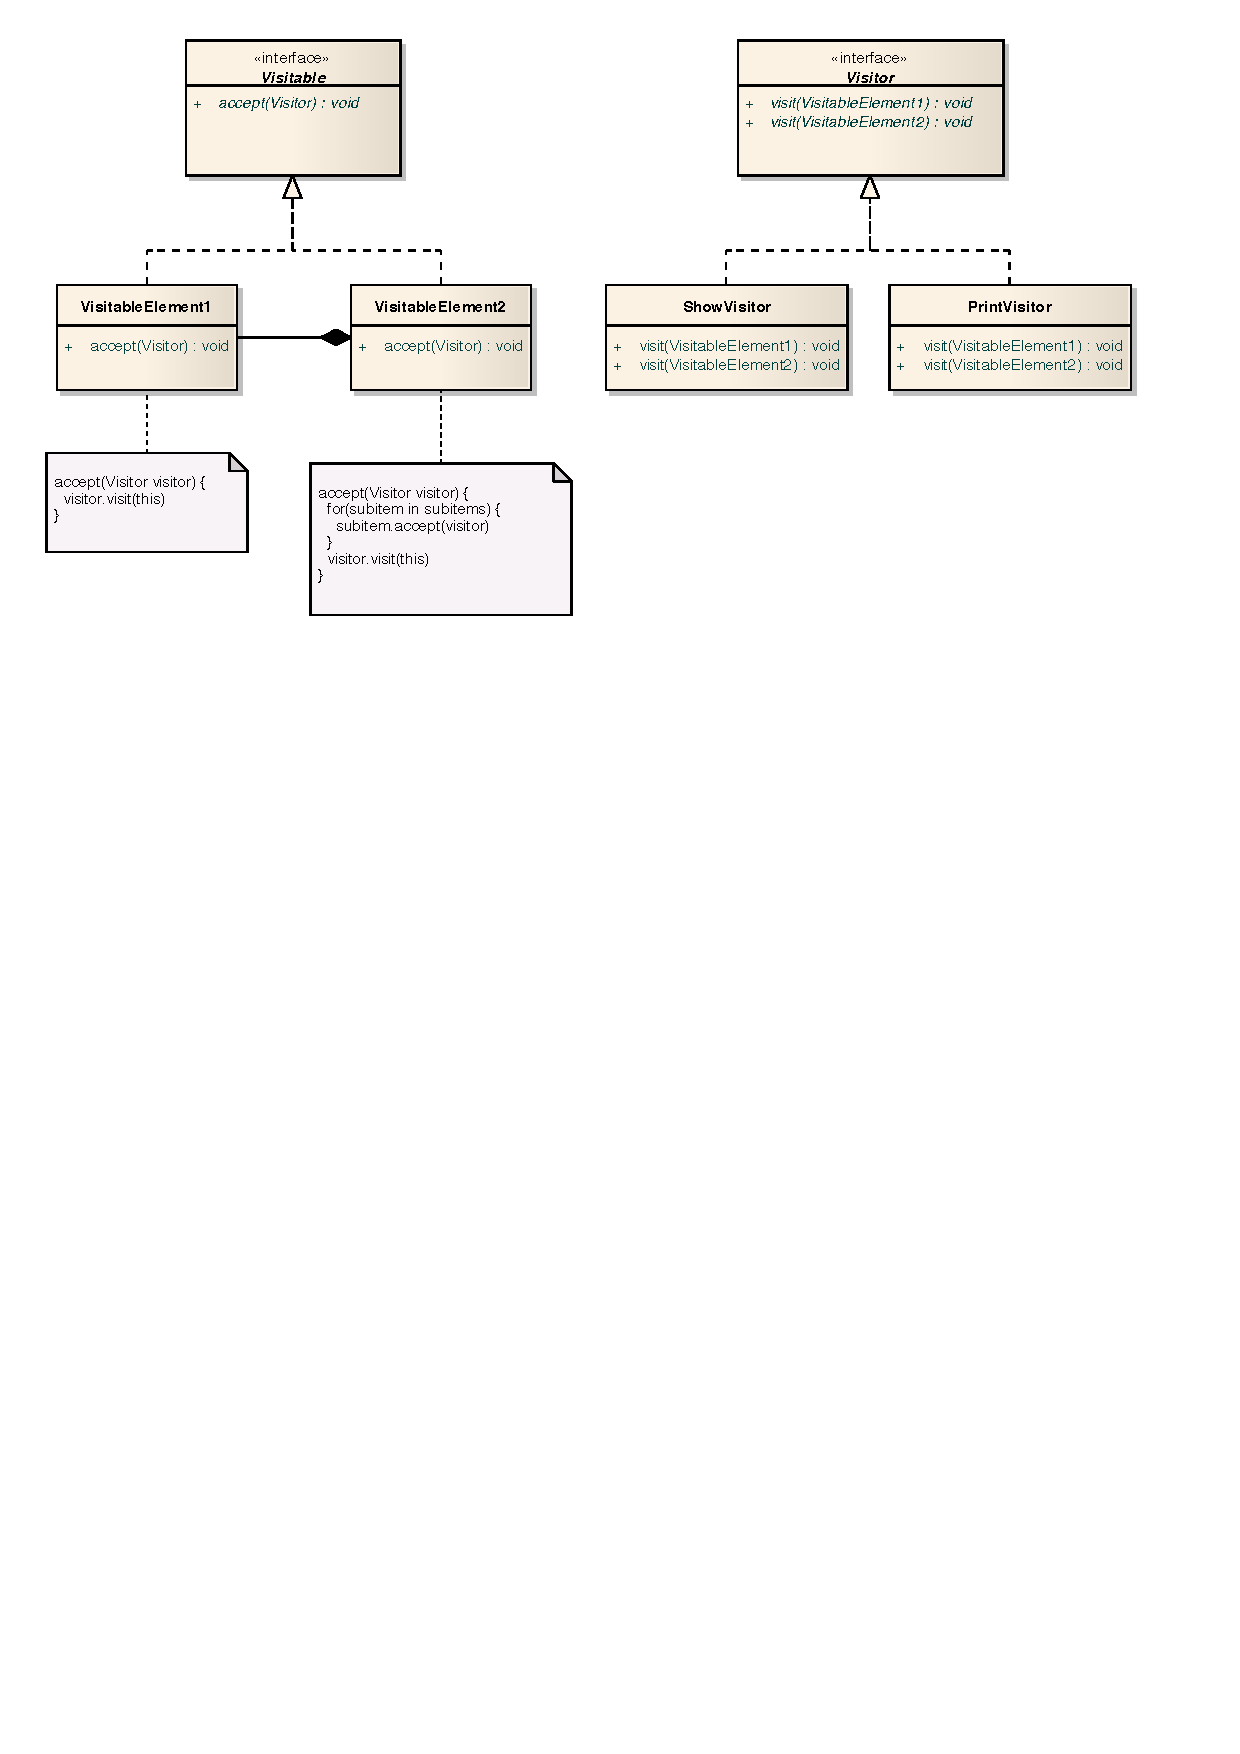
\includegraphics[width=0.9\linewidth]{resources/visitor.pdf}
  \caption[Het \emph{visitor} patroon in UML]{Het \emph{visitor} patroon in UML (Bron: \citep{wikipedia:visitor})}
  \label{fig:visitor}
\end{figure}

Het principe tracht een ontkoppeling te maken van een taxonomie van klassen en
de manier waarop deze klassen overlopen kunnen worden. Het patroon vraagt
daarom het bestaan van twee basis-entiteiten: een te bezoeken taxonomie met een
gemeenschappelijke basisklasse en een declaratie van een bezoekende klasse.

De gemeenschappelijke basisklasse declareert typisch een methode \ttt{accept}
die een instantie van de bezoekende klasse als parameter accepteert. De
bedoeling is dat de implementerende taxonomie vervolgens voor elke klasse
specifiek een implementatie maakt van deze methode. Deze implementatie zal
ofwel de bezoekende klasse doorspelen aan hi\"erarchisch onderliggende klassen,
ofwel een \ttt{visit} methode op de bezoekende klasse oproepen met zichzelf als
argument.

Op een implementatie van een bezoekende klasse kunnen nu verschillende
overladen (Engels: \emph{overloaded}) methoden defini\"eren voor elk van de
klassen in de taxonomie. Op deze manier kan men verschillende bezoekende
klassen realiseren zonder aanpassing aan de bezochte klassen en moet de
bezoekende klasse ook niets afweten van de structuur van de taxonomie.

\section{In Python}

In Python beschikken we echter niet over het concept van overladen functies.
Dit gebrek kan opgevangen worden door het type van de klasse mee op te nemen in
de \ttt{visit} functie. Dit vraagt natuurlijk wel dat ook bij de oproep van de
\ttt{visit\_<type>} functie ook dit type mee in beschouwing wordt genomen. Zo
vervalt wel de mogelijkheid om met \'e\'en implementatie van de functie een
onderliggend deel van de taxonomie te voorzien van een standaard implementatie.
Figuur \ref{fig:py-visitor} geeft de opbouw van een mogelijke implementatie in
Python weer.

\begin{figure}[ht]
  \centering
  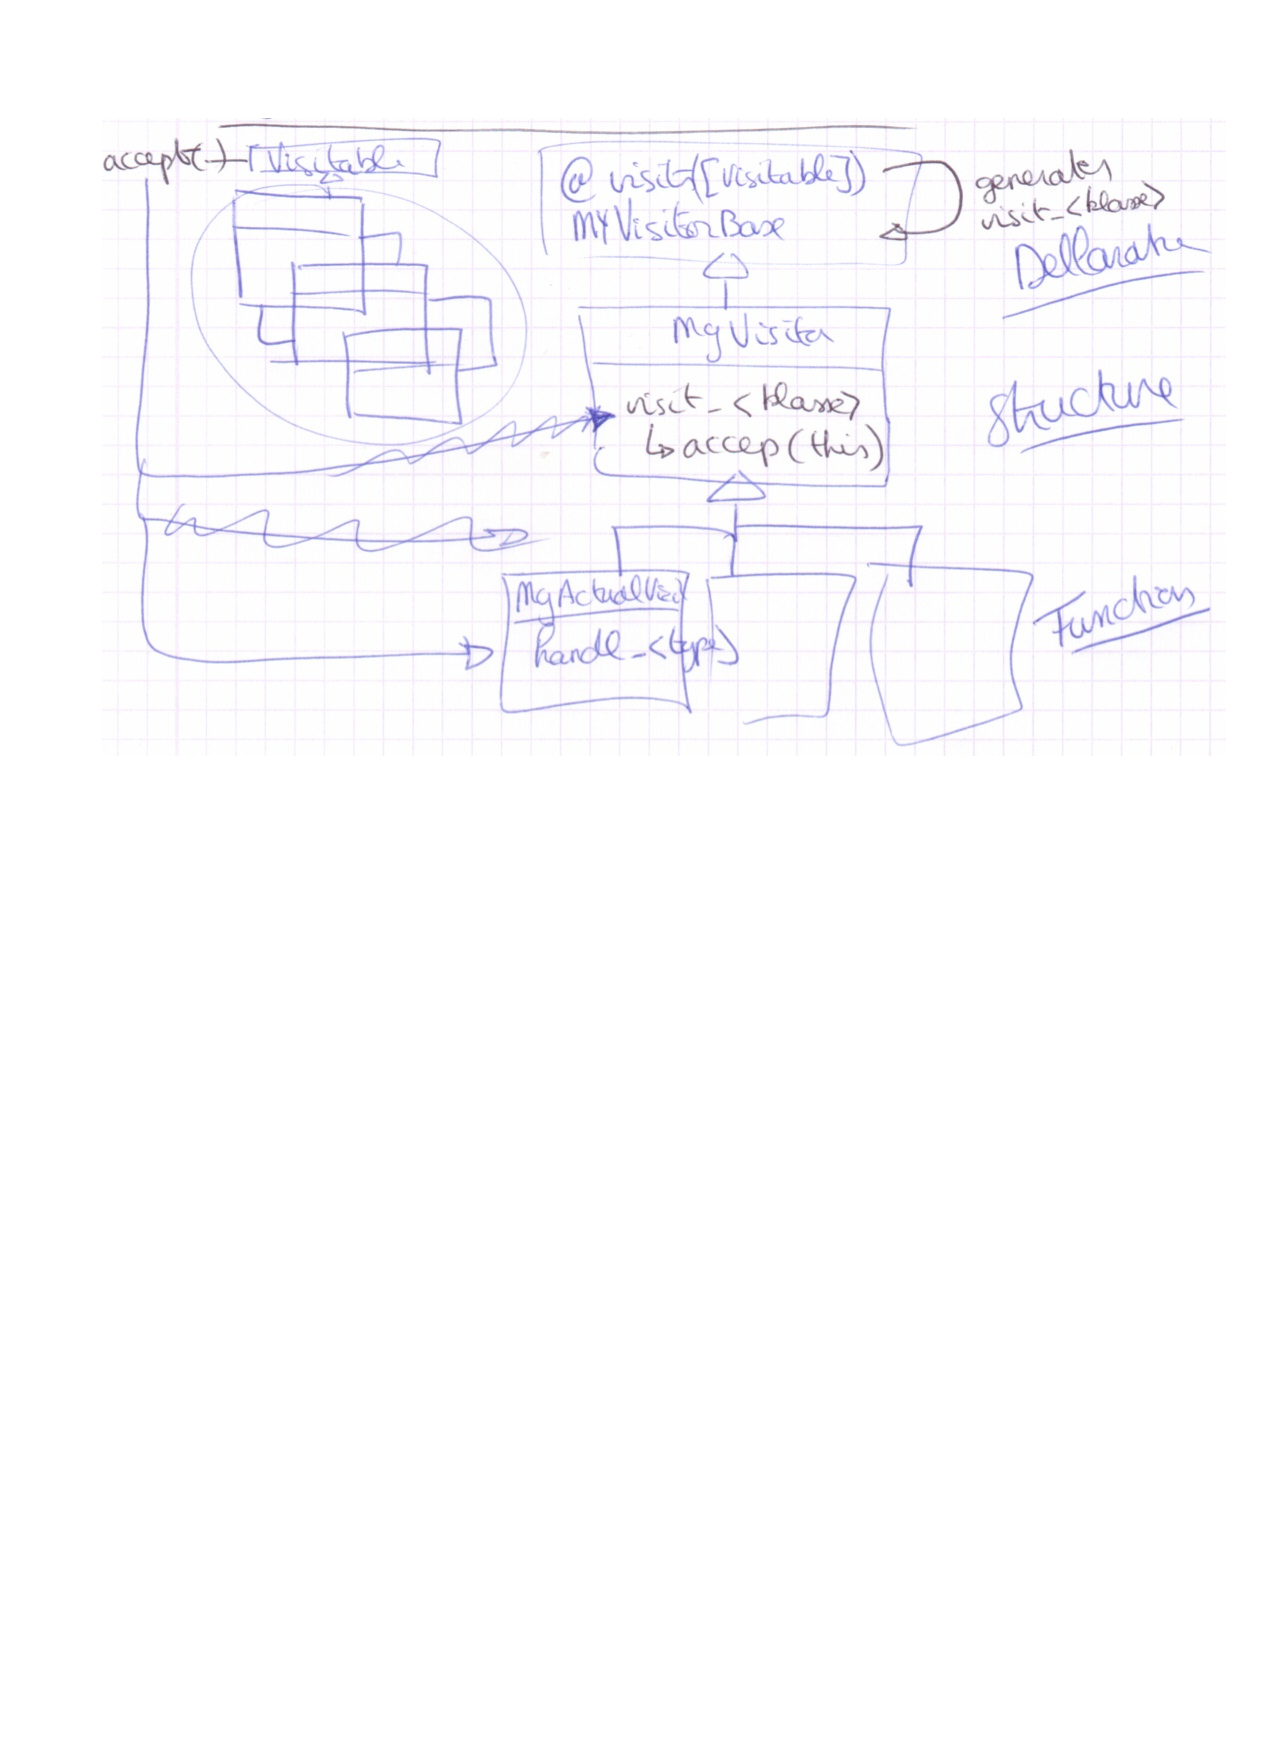
\includegraphics[width=0.9\linewidth]{resources/py-visitor.pdf}
  \caption{Een \emph{visitor} implementatie in Python}
  \label{fig:py-visitor}
\end{figure}

Dankzij het dynamische karakter van Python is het wel mogelijk om veel
van deze problematiek te verbergen en te automatiseren. Door gebruik te maken
van \emph{decorators} is het mogelijk om Python functies en klassen dynamisch
aan te passen voor ze gebruikt worden. Door middel van dit principe is het
mogelijk om een klasse te declareren die de klassen die in een bepaalde module
gedefini\"eerd zijn kan bezoeken en vervolgens een implementatie te maken van
deze klasse die de structuur van de taxonomie implementeert door op dezelfde
manier als in de standaard oplossing een \ttt{accept} functie op te roepen.

Deze \ttt{accept} functie is ge\"implementeerd op een basisklasse voor de
klassen in de taxonomie en gebruikt de introspectieve capaciteiten van Python
om dynamisch een functieoproep te construeren naar een \ttt{handle\_<type>}
functie. Deze functies kunnen ge\"implementeerd worden op een klasse die de
eigenlijke functionaliteit van de \emph{visitor} implementeert en daarvoor
overerft van de eerste concrete implementatie van de \emph{visitor}.

Deze drieledige structuur laat toe om zeer functionele bezoekende
implementaties te maken. Louter de echte functionaliteit wordt opgenomen in een
functie met signatuur \ttt{handle\_<type>}. Deze simpele uitwendige interface
is ook mede de reden dat doorheen de hele implementatie van de generator vele
bezoekende klassen gebruikt worden.

Een laatste bijkomende uitbreiding die ook werd toegevoegd is de opsplitsing
van de \ttt{handle\_<ttype>} functie in een \ttt{before\_visit\_<type>} en
\ttt{after\_visit\_<type>}. Hierdoor de manier waarop doorheen de
hi\"erarchische boomstructuur wordt gelopen bepaald worden: ofwel eerst in de
breedte (Engels: \emph{Depth-First}) ofwel eerst in diepte (Engels:
\emph{Breadth-First}). Dit kan bv. belangrijk zijn indien eerst de
onderliggende kinderen moeten verwerkt worden, vooraleer de feitelijke
transformerende functionaliteit mag toegepast worden. De vertaling van het SM
naar het CM is hiervan een voorbeeld.
